\documentclass[border=10pt]{standalone}

\usepackage{tikz}
\usepackage{tikzsymbols}
\usetikzlibrary{calc,patterns,shapes.geometric}

\def\centerarc[#1](#2)(#3:#4:#5){\draw[#1] ($(#2)+({#5*cos(#3)},{#5*sin(#3)})$) arc (#3:#4:#5);}

\begin{document}
	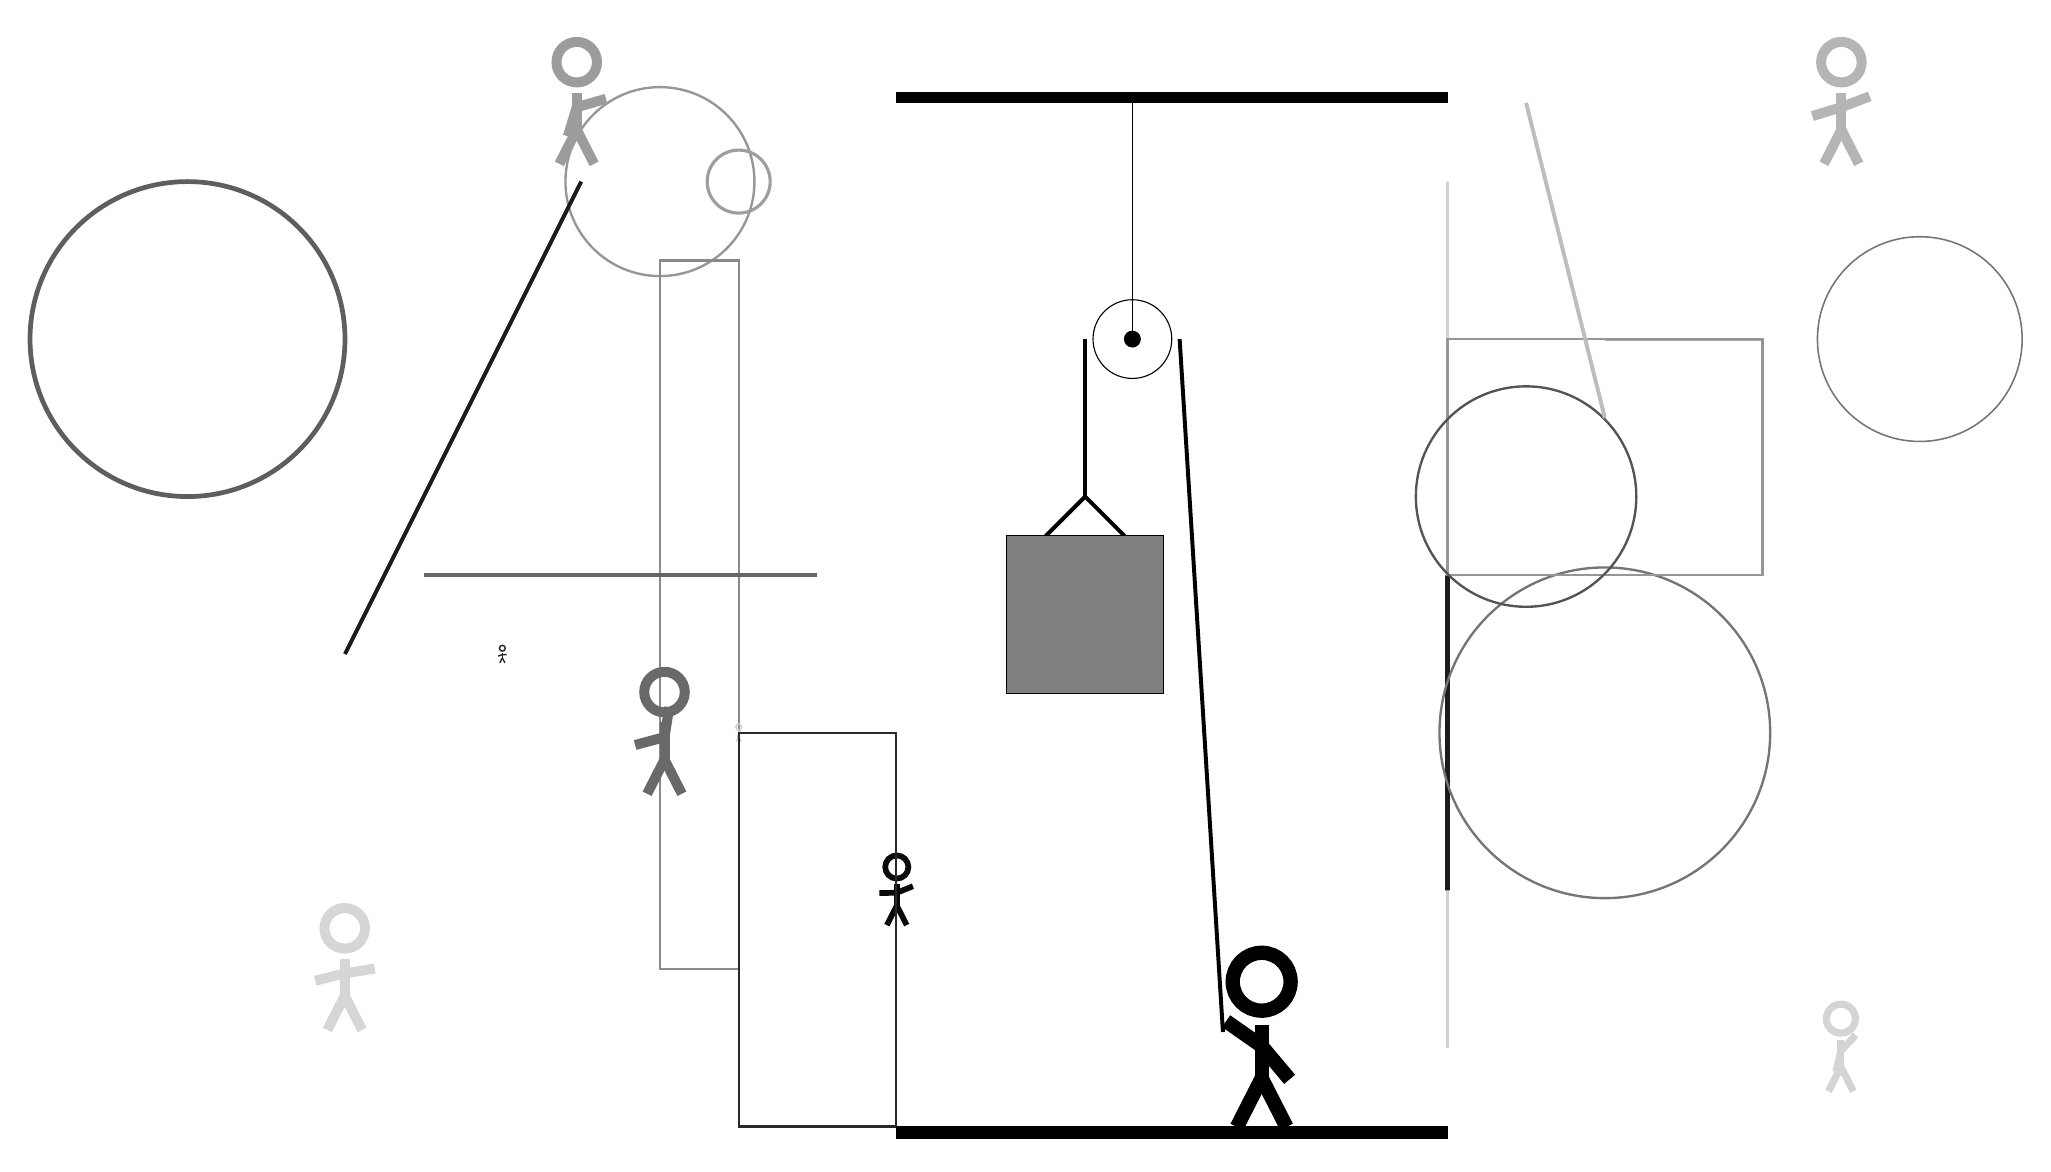
\begin{tikzpicture}
		%%%%% START %%%%%
		
		\draw[fill=black] (-2, 10) rectangle (5, 10.125);
		
		\draw (1, 7) circle (0.5);
		\draw[fill=black] (1, 7) circle (0.1);
		\draw (1, 10) -- (1, 7);
		
		\draw [line width=0.3mm, color=black!41](-5, 9) circle (1.2);
		
		\node[line width=0.6mm, color=black!86] at (-7, 3) {\Strichmaxerl[1][19][2]};
		\draw[line width=0.3mm, color=black!18] (5, -2) rectangle (5, 9);
		\draw[line width=0.3mm, color=black!46] (-4, 8) rectangle (-5, -1);
		
		\node[line width=0.6mm, color=black!19] at (-4, 2) {\Strichmaxerl[1][69][62]};
		
		\node[line width=0.2mm, color=black!59] at (-5, 2) {\Strichmaxerl[7][15][81]};
		
		\draw[line width=0.7mm, color=black!89] (5, 4) rectangle (5, 0);
		
		\draw[line width=0.5mm, color=black!60](-3, 4) -- (-8, 4);
		\node[line width=0.4mm, color=black!16] at (-9, -1) {\Strichmaxerl[7][14][9]};
		\draw [line width=0.2mm, color=black!54](11, 7) circle (1.3);
		\draw [line width=0.3mm, color=black!54](7, 2) circle (2.1);
		
		\node[line width=0.6mm, color=black!96] at (-2, 0) {\Strichmaxerl[4][1][22]};
		\draw[line width=0.4mm, color=black!35] (7, 7) rectangle (9, 7);
		\draw[line width=0.5mm, color=black!89](-6, 9) -- (-9, 3);
		\node[line width=0.3mm, color=black!39] at (-6, 10) {\Strichmaxerl[7][73][16]};
		\draw[line width=0.3mm, color=black!84] (-2, 2) rectangle (-4, -3);
		\draw [line width=0.4mm, color=black!38](-4, 9) circle (0.4);
		\draw[line width=0.3mm, color=black!41] (5, 4) rectangle (9, 7);
		\draw [line width=0.3mm, color=black!67](6, 5) circle (1.4);
		\draw[line width=0.5mm, color=black!26](6, 10) -- (7, 6);
		\draw [line width=0.6mm, color=black!63](-11, 7) circle (2.0);
		
		\node[line width=0.6mm, color=black!29] at (10, 10) {\Strichmaxerl[7][17][21]};
		\node[line width=0.7mm, color=black!17] at (10, -2) {\Strichmaxerl[5][77][47]};
		
		\draw[line width=0.5mm] (-0.1, 4.5) -- (0.4, 5.0) -- (0.9, 4.5);
		\draw[fill=black!50] (-0.6, 4.5) rectangle (1.4, 2.5);
		
		\draw[line width=0.5mm] (0.4, 7) -- (0.4, 5.0);
		\centerarc[line width=0.5mm](1, 7)(0:180:0.6);
		\draw[line width=0.5mm](1.6, 7) -- (2.15, -1.8);
		
		\node at (2.6, -1.9) {\Strichmaxerl[10][-35][-50]};
		
		\draw[fill=black] (-2, -3) rectangle (5, -3.15);
		
		%%%%% END %%%%%
	\end{tikzpicture}
\end{document}